\newpage
%%%%%%%%%%%%%%%%%%%%%%%%%%%%%%%%%%%%%%%%%%%%%%%%%%%%%%%%%%%%%%%%%%%%%%%%%%%%%%%
\section{Week 5}
%%%%%%%%%%%%%%%%%%%%%%%%%%%%%%%%%%%%%%%%%%%%%%%%%%%%%%%%%%%%%%%%%%%%%%%%%%%%%%%
\subsection*{I can't be asked}
\begin{itemize}
    \item I am too lazy to summarize my shitty git commits from the 13 til now
        (the 31st).
    \item Enjoy Mr. Incredible Uncanny 4 instead:
    \begin{figure}[ht]
        \centering
        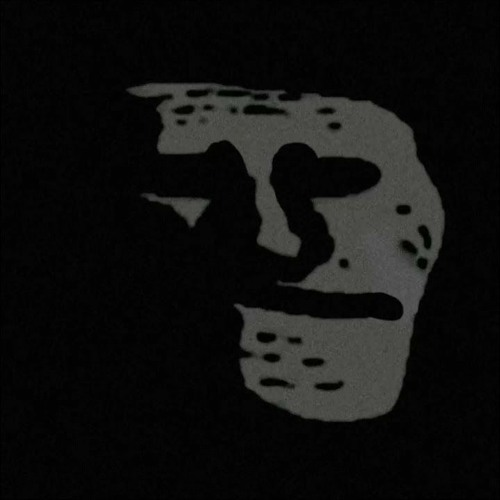
\includegraphics[width=6cm]{uncanny4}
        \captionsetup{labelfont=bf, textfont=it}
        \caption{oooooooooooooooooooo}
        \label{fig:uncanny4}
    \end{figure}
    \item Right, now I've added a few things:
        \begin{itemize}
            \item custom link style and formatting in casts 
            \item render images in casts
            \item sign in with farcaster (doesn't do much else yet)
            \item link to view cast on warpcast 
        \end{itemize}
    \item I suppose I should add reaction data and stuff now.
    \item I'm avoiding the actual hard tech of having the LLM not hallicinate.
        I'm thinking of having a writers room where my proprietary spagetti code
        strips out the things that don't make logical sense from the summary
        from the LLM.
\end{itemize}
\clearpage
\subsection*{I really can't be asked}
\begin{itemize}
    \item I suck at updating this, but I'm focused on a native farcon app at the
        moment. you can check it out
        \textcolor{blue}{\href{https://farcon.info}{here}}.
    \item I'm trying to get messaging working by handcrafting endpoints in rust
        (this will be my downfall, I should just use Neynar) so I'll use them in
        both apps anyways.
    \item Figure~\ref{fig:farcaster_auth} is a drawing (from farcaster YT 
        tutorial) which shows how to create a message with a custom client 
        application.
        \begin{figure}[ht]
            \centering
            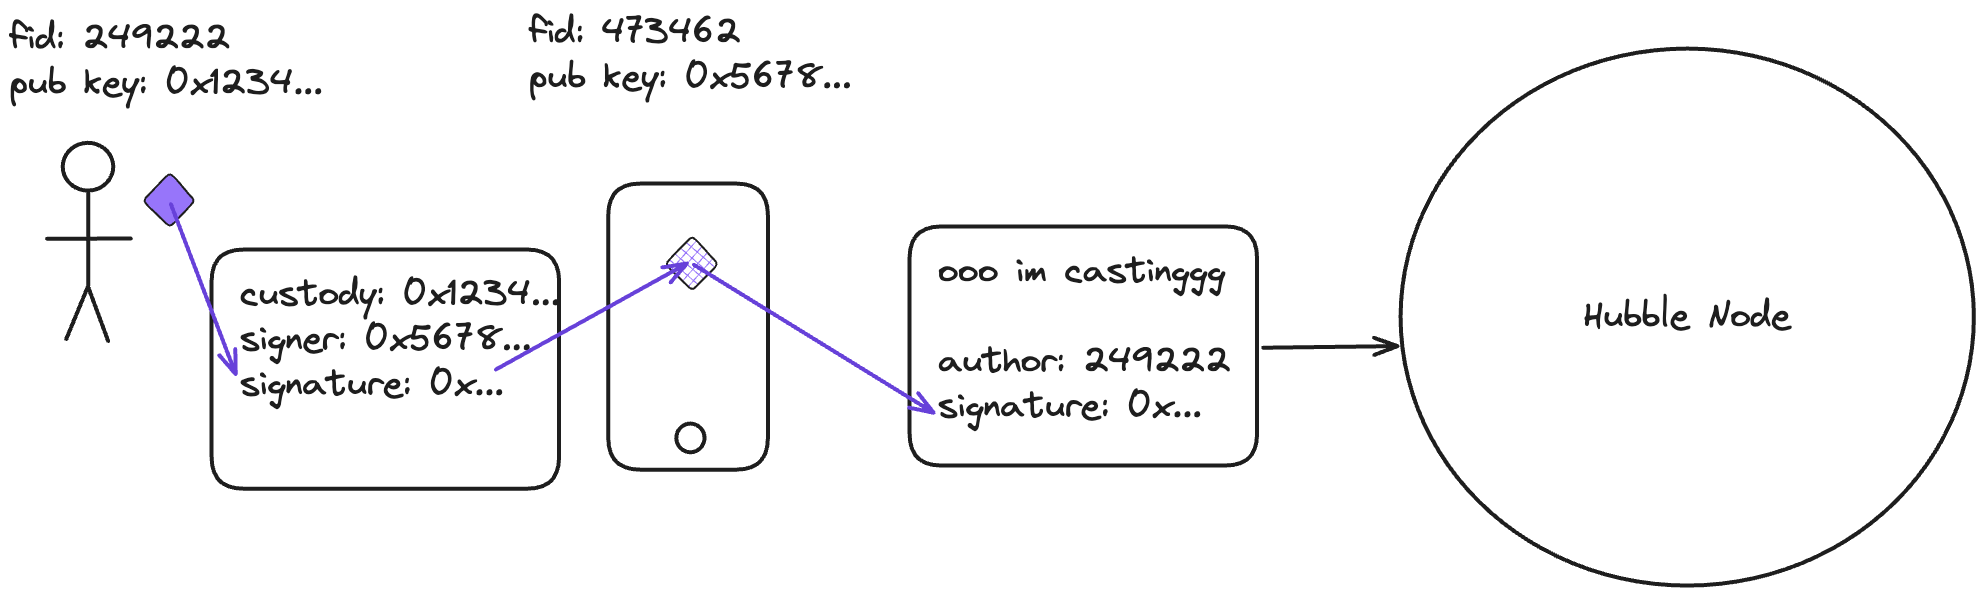
\includegraphics[width=15cm]{farcaster_auth}
            \captionsetup{labelfont=bf, textfont=it}
            \caption{Farcaster Signer Concept}
            \label{fig:farcaster_auth}
        \end{figure}
\end{itemize}

